\documentclass[journal]{IEEEtran}
\IEEEoverridecommandlockouts
% The preceding line is only needed to identify funding in the first footnote.
%If that is unneeded, please comment it out. \usepackage{cite}
\usepackage{amsmath,amssymb,amsfonts}
\usepackage{algorithmic}
\usepackage{graphicx}
\usepackage{textcomp}
\usepackage[x11names]{xcolor}
\usepackage{listings}
\usepackage{float}
\usepackage{tikz}
\usepackage{siunitx}
\usepackage{amsmath}
\usepackage{todonotes}
\usepackage[backend=biber, style=ieee]{biblatex}

\usetikzlibrary{graphs}
\usetikzlibrary {arrows.meta}
\usetikzlibrary{calc}
\usetikzlibrary {shapes.multipart}

\input{listings_python_style.tex}


\addbibresource{bib.bib}
\begin{document}

\title{Mobile Computing Laboratory 2021\\
Assignment Report}

\author{\IEEEauthorblockN{Tobias Lafer}
\IEEEauthorblockA{\textit{Technical University of Graz}, Austria}}

\maketitle

\begin{abstract}
    In the \textit{Mobile Computing}-laboratory, at TU Graz, the students learn
    in a hands-on way the fundamentals of developing applications for
    state-of-the-art mobile computing devices. As a final result, the students
    create an Android-application for either a pre-defined (for beginners) or a
    self-chosen (for experienced students) task. Due to the missing experience
    app-development, the pre-defined task was chosen by the
    author.\newline
    This document describes and discusses the essential ideas and concepts of
    the developed app as well as the derived performance and the raised issues. \newline
    The source-code of the app as well as the data-set and all additional scripts etc. can 
    be found on \cite{lafer_mobile-computing_2021}.
\end{abstract}

\section{Introduction}
The pre-defined task is divided into two parts: First, activity-monitoring based
on a rather simple classifier, like \textit{k-nearest-neighbors (kNN)}, and
secondly, phone-position independent activity monitoring through on-device
transfer-learning.\newline
In more detail: A set of activities should be chosen by the student and a
simple-classifier should be designed to distinguish certain activities via the
captured sensor-data on the device. Thereby, the required data-set for training
the classifier should be self-captured. 
For the second part, a pre-captured data-set for similar should be used to
design a neural-network based classifier. Using transfer-learning, this
classifier should then be trained on a smaller, on-device captured data-set for
the current phone-position.\newline
To ease the app-development, a software-library was provided implementing
the transfer-learning procedure itself \cite{pavel_senchanka_example_2019} to let
the students focus on developing the classifier itself as well as the necessary
signal capturing and pre-processing. 

\section{\textit{kNN}-classification} 
The \textit{k-nearest-neighbors}-algorithm \cite{noauthor_k-nearest_2021} is a
simple but very powerful classification algorithm, based on a majority-voting of
the distances between the current individual to classify and a set of labeled
reference-individuals. Therby, no formal restrictions on the distance
measurement are given (one can even define its own 'distance'), but typically
one uses a certain type of \textit{norm} \cite{noauthor_norm_2021}, mostly the
well-known \textit{euclidean norm} \cite{noauthor_euclidean_2021}. After
calculating the distances, one sorts them in ascending order and counts the
classes of the $k$ first distances. Therby, $k$ is an design-parameter which
has to be properly chosen. The final class of the individual is then the one with the
highest count of this $k$ closest reference-individuals.\newline
Listing \ref{kNN_listing} shows a \textit{Python}-implementaion of kNN. The
classifier implemented in the app is also based on this code.\newline


\begin{lstlisting}[language=iPython, label=kNN_listing, captionpos=b,caption=A simple python-implementation of \textit{kNN}.]
def kNN(features_in, features_ref, labels_ref, 
        k, N_classes): 

    differences = features_ref - features_in 
    euclidian_distances = 
        np.linalg.norm(differences, axis=1) 
    sorted_indices = np.argsort(euclidian_distances) 
    sorted_labels = labels_ref[sorted_indices]
    
    return k_majority_voting(sorted_labels, N_classes, k)
    
def k_majority_voting(data, k, N_classes): 
    counters = np.zeros((N_classes), dtype=int) 

    for l in range(k): 
        counters[data[l]] += 1
        
    sorted_indices = np.argsort(counters) 
    return sorted_indices[-1]
\end{lstlisting}



\section{Activities for the \textit{kNN}-classification} 
Four well-known body-strength exercises were chosen as activities to be classified.
These activities were selected as each of them has a quite unique 
motion-profile, and were therefore supposed to be easily distinguishable by 
\textit{kNN}. A sketch of each activity is shown in figures 
\ref{ref:fig_kNN_activity_1} to \ref{ref:fig_kNN_activity_4}. 
Thereby, the phone is placed as shown in figure \ref{fig:knn_position}.

\begin{figure}[H]
    \begin{minipage}[t][3.5cm][b]{0.11\textwidth}
        \begin{figure}[H]
            \centering
            \includegraphics[width=\textwidth]{figures/curls.png}
            \caption{Bizeps\\Curls \cite{noauthor_notitle_2021-3}}
            \label{ref:fig_kNN_activity_1}
        \end{figure}
    \end{minipage}
    \begin{minipage}[t][3.5cm][b]{0.1\textwidth}
        \begin{figure}[H]
            \centering
            \includegraphics[width=\textwidth]{figures/triceps.png}
            \caption{Triceps\\Curls \cite{noauthor_notitle_2021}}
            \label{ref:fig_kNN_activity_2}
        \end{figure}
    \end{minipage}
    \begin{minipage}[t][3.5cm][b]{0.12\textwidth}
        \begin{figure}[H]
            \centering
            \includegraphics[width=\textwidth]{figures/crunch.png}
            \caption{Crunches\\\cite{noauthor_notitle_2021-1}}
            \label{ref:fig_kNN_activity_3}
        \end{figure}
    \end{minipage}
    \begin{minipage}[t][3.5cm][b]{0.11\textwidth}
        \begin{figure}[H]
            \centering
            \includegraphics[width=\textwidth]{figures/russian-twist.jpg}
            \caption{Russian-Twist \cite{noauthor_notitle_2021-2}}
            \label{ref:fig_kNN_activity_4}
        \end{figure}
    \end{minipage}
\end{figure}
\begin{figure}[htbp]
    \centering
    \includegraphics[width=0.4\textwidth]{figures/kNN_position.png}
    \caption{Phone position as used for the \textit{kNN}-classification task.}
    \label{fig:knn_position}
\end{figure}

\section{Signal processing}
The data from both, accelerometer and gyroscope sensors of the phone, 
are continuously captured in an
event-based manner (see \cite{noauthor_sensoreventcallback_2021}). The actual
classification is then executed with a period of one second in separate thread. 
A sketch of the corresponding signal-processing pipeline is shown in figure
\ref{fig:kNN_signal_processing}.

\begin{figure}[htbp]
    \centering
    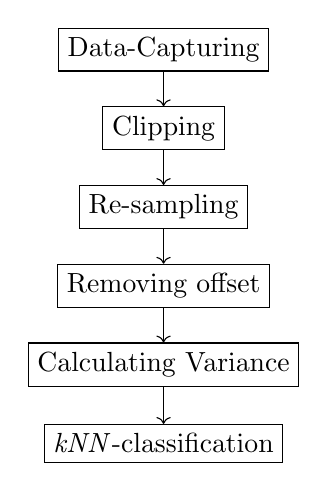
\begin{tikzpicture}
        \node[draw] (capturing) at (0,0) {Data-Capturing}; \node[draw]
        (clipping) at (0,-1) {Clipping}; \node[draw] (resampling) at (0,-2)
        {Re-sampling}; \node[draw] (offset) at (0,-3) {Removing offset};
        \node[draw] (energies) at (0,-4) {Calculating Variance}; \node[draw]
        (kNN) at (0,-5) {\textit{kNN}-classification};

        \graph[nodes={draw}] {(capturing) -> (clipping) -> (resampling) ->
            (offset) -> (energies) -> (kNN);};
    \end{tikzpicture}
    \caption{Outline of signal-processing pipeline.}
    \label{fig:kNN_signal_processing}
\end{figure}

\begin{enumerate}
    \item \textbf{Data-Capturing}\newline
        The Android operating-system offers classes and routines to handle the
        event-based capturing of on-device sensor-signals 
        \cite{noauthor_sensoreventcallback_2021}. Thereby, an event is
        triggered each time one of the registered sensors delivers new values.
        The derived $x$-, $y$- and $z$- signals per sensor are then
        pushed to fix-sized buffers including their timestamps. 
        If a buffer buffer is full, the oldest values are removed from it when 
        pushing the new ones.
    \item \textbf{Clipping}\newline
        It was found that a time-period of $4$ seconds is enough
        to classify the selected activities. Therefore, the time-series 
        contained in the capturing buffers are clipped to this period.
    \item \textbf{Resampling}\newline
        Next, the clipped time-series are re-sampled to a uniform sampling rate
        of $50\ \si{\hertz}$ by linear interpolation between the two
        neighbor samples. Each sensor-channel then contains exactly $200$
        samples.
    \item \textbf{Offset removal}\newline
        The activities to monitor are periodic, so only the AC-part of the
        single timeframes are required.
    \item \textbf{Variance calculation}\newline
        The actual features used for classification are the variances of the
        single sensor-channels:
        \begin{align}
            \mathit{var}\left(\{x_{i,k}\}\right) = \frac{1}{N} \sum\limits_{k=0}^{N-1} x_{i,k}^2 \quad \forall i = 1 ... 6
        \end{align}
    \item \textbf{\textit{kNN}-classification}\newline
        The previously calculated variances are then fed into the
        \textit{kNN}-algorithm using $k=10$. The \textit{euclidean norm} is used
        as distance-measurement.
\end{enumerate}

\section{Applying actual data to \textit{kNN}} 
A set of samples for each activity was captured and split into the required 
$4$ seconds timeframes, each overlaping for $3$ seconds. 
The data-set was separated into a 'training' and a 'validation'-set, 
with a validation-split of $25\ \si{\percent}$. 
The distributions of the single activities in both sub-sets are shown in
figures  \ref{fig:hist_kNN_training} and \ref{fig:hist_kNN_validation}.

\begin{figure}[H]
    \centering
    \includegraphics[width=0.3\textwidth]{figures/hist_kNN_training.eps}
    \caption{Activity-histogram of the training-set.}
    \label{fig:hist_kNN_training}
\end{figure}

\begin{figure}[H]
    \centering
    \includegraphics[width=0.3\textwidth]{figures/hist_kNN_validation.eps}
    \caption{Activity-histogram of the validation-set.}
    \label{fig:hist_kNN_validation}
\end{figure}

If an clear distinction between the 4 different classes is actually possible via
\textit{kNN} can be investigated by a so-called \textit{pair-plot} \cite{noauthor_seabornpairplot_2021}. 
Thereby, a set of sub-plots is generated and set up in way to unroll the, 
in this case, 6-dimensional feature-vectors in a 2D plot pane. 
The pair-plots for both, training and validation sets are shown
in figures \ref{fig:pairplot_kNN_training} and
\ref{fig:pairplot_kNN_validation}. 
The off-diagonal plots are of main interest, as these plots
show the relationships between one selected feature and all remaining features.
If a clear grouping is visible in one of the plots, the corresponding
feature-pair can be used for classification.


\begin{figure}[htbp]
    \centering
    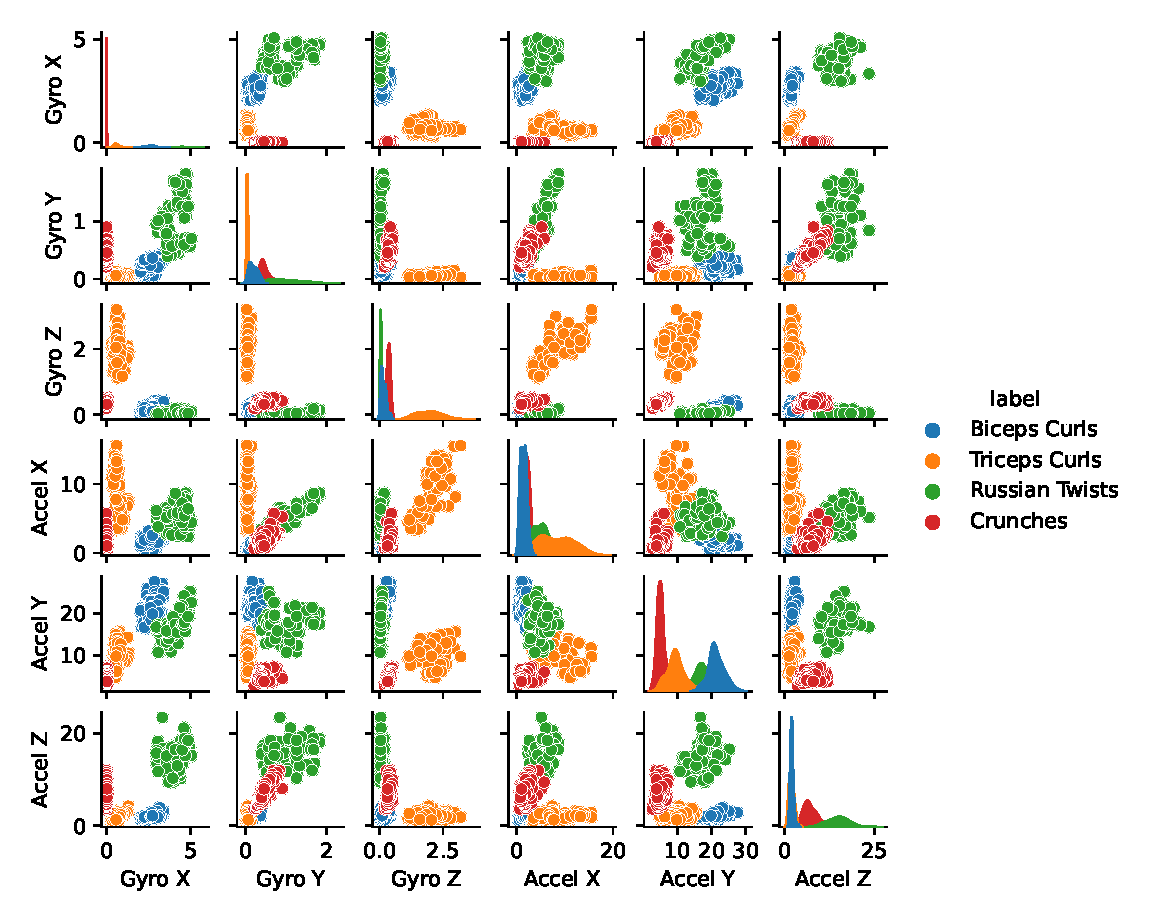
\includegraphics[width=0.5\textwidth]{figures/kNN_pairplot_training.eps}
    \caption{Pair-plot of the training-set.}
    \label{fig:pairplot_kNN_training}
\end{figure}

\begin{figure}[htbp]
    \centering
    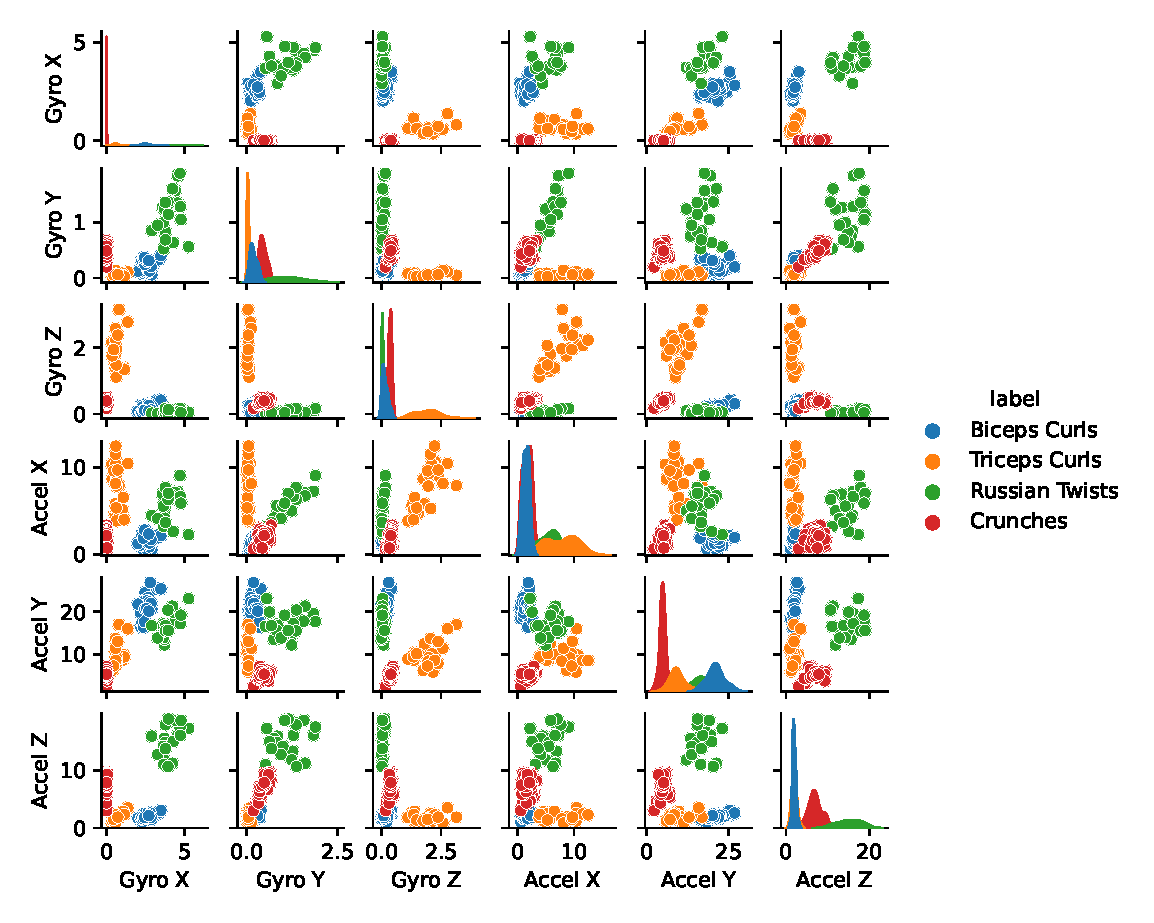
\includegraphics[width=0.5\textwidth]{figures/kNN_pairplot_validation.eps}
    \caption{Pair-plot of the validation-set.}
    \label{fig:pairplot_kNN_validation}
\end{figure}

The performance of the classifier can nicely be visualized by a so-called
'confusion-matrix'. Therby, the samples from the validation-set are consecutively 
fed into the \textit{kNN}-classifier. The predicted and correct classes are then 
plotted in a 2D grid. A perfect classifier contains only elements on the main-diagonal
grid faces.\newline
Due to the quite clear grouping visible in the pari-plots a clear distinction
between the activities can be assumed. The proof of this assumption is given
by the confusion-matrix in figure \ref{fig:kNN_confusion}, where one can observe
that all samples were classified correctly.

\begin{figure}[htbp]
    \centering
    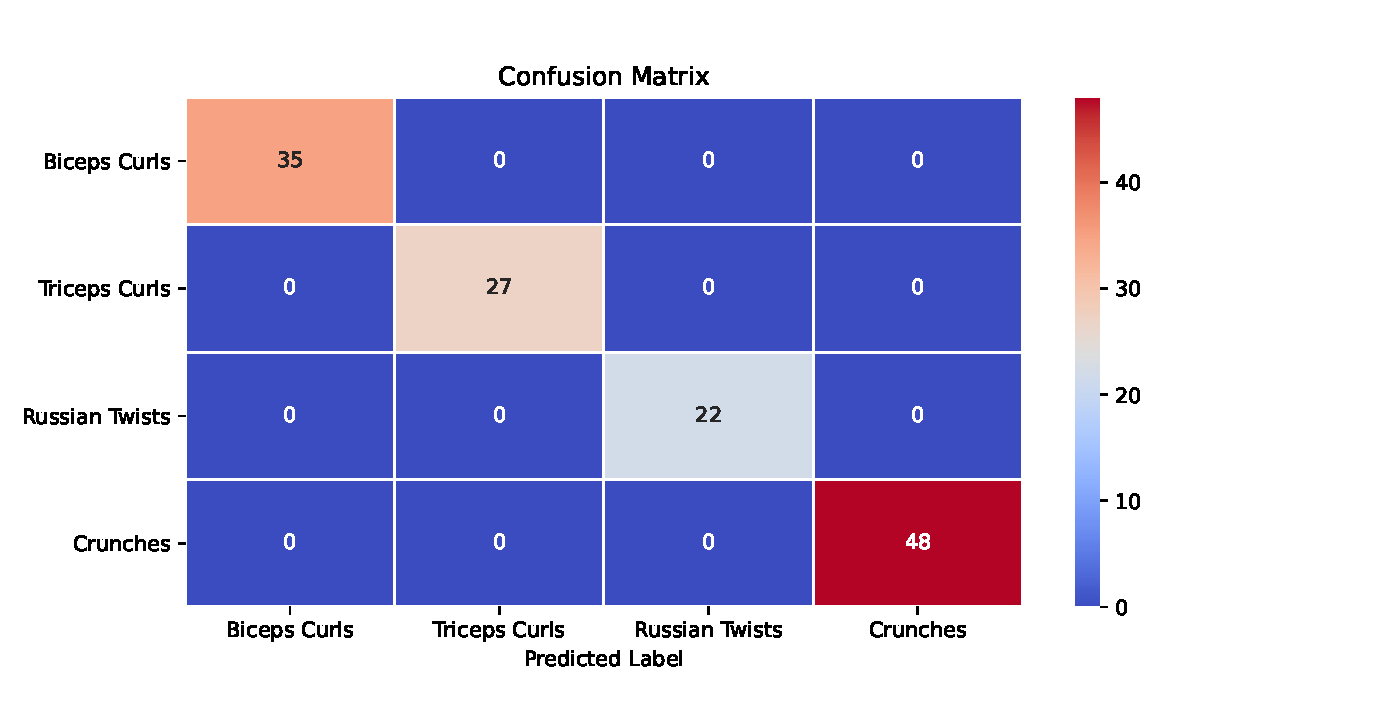
\includegraphics[width=0.5\textwidth]{figures/kNN_confusion_matrix.eps}
    \caption{Confusion-matrix for the \textit{kNN}-classifier.}
    \label{fig:kNN_confusion}
\end{figure}




\section{Transfer-learning basics}
Changing the phone's position when attempting to classify an activity will
typically lead to a massive drop in accuracy, although the underlying activity
is the same. \textit{Transfer learning} is one solution to this issue. Thereby,
an existing machine-learning model, the so-called \textit{parent-model}, 
typically trained on a huge data-set, is slightly modified and re-trained on a 
new but typically smaller data-set.
If both, old and new
data-sets, are somehow related to each other (e.g. same activities but different
phone positions), one could derive similar classification performance, but
without designing and training a model from scratch.\newline
In the second part of this assignment a neural-network is used for
classification, trained on a large
data-set for one dedicated phone-position. Afterwards, the output-layer as well as
some of the top hidden layers are removed and a new, so-called \textit{head-model},
is attached to the remaining parts of the parent-model. Throughout the rest of this
paper, the remaining parts of the parent in the child-model is called \textit{base-model}.
 The parameters of the base-model are fixed so that only
the head of this new \textit{transfer-learning model} (\textit{TFL}-model) is
trained for a new phone-position \textbf{on-device}.

\section{Activities, Data-set and Model-architecture}
Due to several issues during development and with first phone
used in this assignment, a totally different set of activities
were used for the second part. Further, no pre-captured data-set was used,
but the author captured the data-sets for both, parent and child-models himself.
The reasons for this decisions are discussed in detail in section \ref{sec:conclusion}.\newline

The following activities were chosen to be classified:
\begin{itemize}
    \item Walking on a plane surface
    \item Walking Upstairs
    \item Walking Downstairs
    \item Running
\end{itemize}

The parent-model is designed for the phone being placed in the front-left
trouser pocket with an orientation as shown in figure \ref{fig:tfl_base}.
Although universally placeable, the phone was placed on the front-right pocket as 
shown in figure \ref{fig:tfl_tfl} for validating the child-model.
Data-sets were captured for both phone-positions and split into
training- and validation-sets using again a validation-split of 
$25\ \si{\percent}$. The corresponding histograms are shown in 
figures \ref{fig:hist_parent_training} to \ref{fig:hist_child_validation}.
 \newline
The actual model architectures for both, parent and head-model are shown in
figures \ref{fig:parent-model} and \ref{fig:head-model}. The essential part of the
parent model is a 2D convolution layer, depicted in more detail in figure
\ref{fig:conv_2d_arch}. \newline
The transfer-learning part utilizes a similar signal
pre-processing scheme as for the \textit{kNN}-classifier 
(see figure \ref{fig:TFL_signal_processing}). Thereby, time-frames
with a length of $4$ seconds are resampled by linear-interpolation to a
sampling-rate of $50\ \si{\hertz}$, resulting in a total of $N_{Samples} = 200$
samples of each of the $6$ available sensor channels. Each channel is then 
normalized by 
\begin{align}
    \{\overset{\wedge}{x}_{i,k}\} = \frac{1}{\mathit{max}\left(\{|x_{i,k}|\}\right)}\{x_{i,k}\}\quad \forall i = 1 ... 6
\end{align}

The resulting $\left(N_{Samples}
\times 6\right)$-matrix is then fed into a 2D convolution layer, setting up
one 2D convolution kernel for each of the 4 activities. The idea behind this
architecture is that each activity is characterized by one or another unique
motion pattern in the sensor-channels. As there is one kernel available for
each activity, the layer has the ability to derive one optimal kernel for each
activity. The pooling-layer following the convolution-layer then just reduces the
number of samples fed into the final dense-layers to reduce the number of tunable parameters. 
By a try-and-error approach,
it was found that the higher the number of neurons in this dense-layers, the
better the accuracy on the validation set. As the parent-model is not trained on
the device directly, a quite high number of neurons was chosen. The head-model for
transfer-learning, on the other hand, has the same base-architecture as the head of
the parent-model, but utilizes a smaller number of neurons to speed-up on-device
training.\newline
All layers except the output-layers of both models use \textit{ReLU}-activation.
As the basic task of this model is a classification-task,
\textit{softmax}-activations are used for the output layers.

\begin{figure}[htbp]
    \centering
    \includegraphics[width=0.45\textwidth]{figures/original_model_position.png}
    \caption{Phone-position for the parent-model data-set.}
    \label{fig:tfl_base}
\end{figure}

\begin{figure}[htbp]
    \centering
    \includegraphics[width=0.45\textwidth]{figures/transfer_learning_position.png}
    \caption{Phone-position for transfer-learning.}
    \label{fig:tfl_tfl}
\end{figure}

\begin{figure}[htbp]
    \centering
    \includegraphics[width=0.3\textwidth]{figures/hist_parent_training.eps}
    \caption{Activity-histogram of the parent-model training-set.}
    \label{fig:hist_parent_training}
\end{figure}

\begin{figure}[htbp]
    \centering
    \includegraphics[width=0.3\textwidth]{figures/hist_parent_validation.eps}
    \caption{Activity-histogram of the parent-model validation-set.}
    \label{fig:hist_parent_validation}
\end{figure}


\begin{figure}[htbp]
    \centering
    \includegraphics[width=0.3\textwidth]{figures/hist_child_training.eps}
    \caption{Activity-histogram of the child-model training-set.}
    \label{fig:hist_child_training}
\end{figure}

\begin{figure}[htbp]
    \centering
    \includegraphics[width=0.3\textwidth]{figures/hist_child_validation.eps}
    \caption{Activity-histogram of the child-model validation-set.}
    \label{fig:hist_child_validation}
\end{figure}

\begin{figure}[htbp]
    \centering
    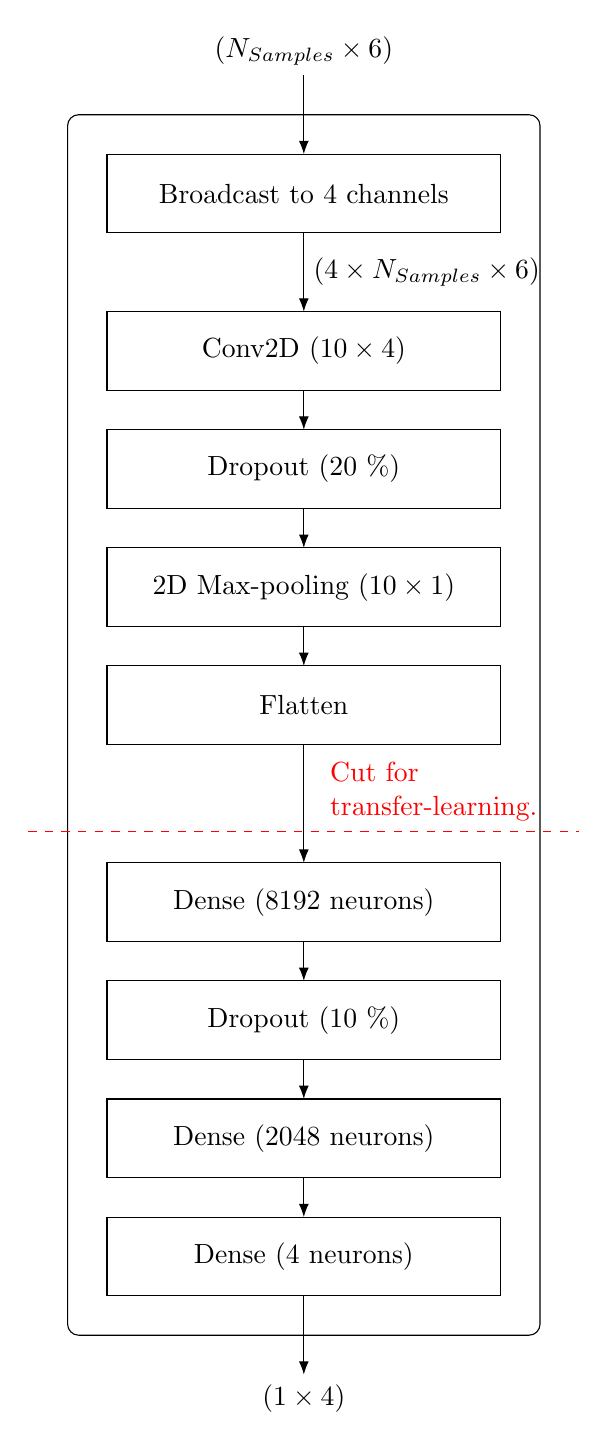
\begin{tikzpicture}
        \draw[rounded corners] (0,0) rectangle (6,-15.5); \draw[Latex-] (3,-0.5)
        -- ++(0,1) node[above] {$\left(N_{Samples} \times 6\right)$};


        \draw (0.5,-0.5) coordinate (tmp) rectangle ++(5,-1); \node () at
        ($(tmp) + (2.5, -0.5)$) {Broadcast to $4$ channels};

        \draw[-Latex] ($(tmp) + (2.5,-1)$) -- ++(0,-1); \node[right] () at
        ($(tmp) + (2.5,-1.5)$) {$\left(4\times N_{Samples}\times 6\right)$};

        \draw (0.5,-2.5) coordinate (tmp) rectangle ++(5,-1); \node () at
        ($(tmp) + (2.5, -0.5)$) {Conv2D ($10\times 4$)};

        \draw[-Latex] ($(tmp) + (2.5,-1)$) -- ++(0,-0.5);

        \draw (0.5,-4) coordinate (tmp) rectangle ++(5,-1); \node () at ($(tmp)
        + (2.5, -0.5)$) {Dropout ($20\ \si{\percent}$)};

        \draw[-Latex] ($(tmp) + (2.5,-1)$) -- ++(0,-0.5);

        \draw (0.5,-5.5) coordinate (tmp) rectangle ++(5,-1); \node () at
        ($(tmp) + (2.5, -0.5)$) {2D Max-pooling $\left(10\times 1\right)$};

        \draw[-Latex] ($(tmp) + (2.5,-1)$) -- ++(0,-0.5);

        \draw (0.5,-7) coordinate (tmp) rectangle ++(5,-1); \node () at ($(tmp)
        + (2.5, -0.5)$) {Flatten};

        \draw[-Latex] ($(tmp) + (2.5,-1)$) -- ++(0,-1.5); \draw[red, dashed]
        ($(tmp) + (-1,-2.1)$) -- ++(7,0); \node[right, text=red] () at ($(tmp) +
        (2.5,-1.6)$) {
                \begin{tabular}{l}
                    Cut for \\ transfer-learning. \end{tabular} };

        \draw (0.5,-9.5) coordinate (tmp) rectangle ++(5,-1); \node () at
        ($(tmp) + (2.5, -0.5)$) {Dense ($8192$ neurons)};

        \draw[-Latex] ($(tmp) + (2.5,-1)$) -- ++(0,-0.5);

        \draw (0.5,-11) coordinate (tmp) rectangle ++(5,-1); \node () at ($(tmp)
        + (2.5, -0.5)$) {Dropout ($10\ \si{\percent}$)};

        \draw[-Latex] ($(tmp) + (2.5,-1)$) -- ++(0,-0.5);

        \draw (0.5,-12.5) coordinate (tmp) rectangle ++(5,-1); \node () at
        ($(tmp) + (2.5, -0.5)$) {Dense ($2048$ neurons)};

        \draw[-Latex] ($(tmp) + (2.5,-1)$) -- ++(0,-0.5);

        \draw (0.5,-14) coordinate (tmp) rectangle ++(5,-1); \node () at ($(tmp)
        + (2.5, -0.5)$) {Dense ($4$ neurons)};

        \draw[-Latex] ($(tmp) + (2.5,-1)$) -- ++(0,-1) node[below]
        {$\left(1\times 4\right)$};
        
        
    \end{tikzpicture}
    \caption{The architecture of the parent-model. All layers except the last
    one use \textit{ReLU}-activation. The output-layer uses
    \textit{softmax}-activation. The architecture of the \textit{Conv2D}-layer is
    shown in detail in figure \ref{fig:conv_2d_arch}.}
    \label{fig:parent-model}
\end{figure}

\begin{figure}[htbp]
    \centering
    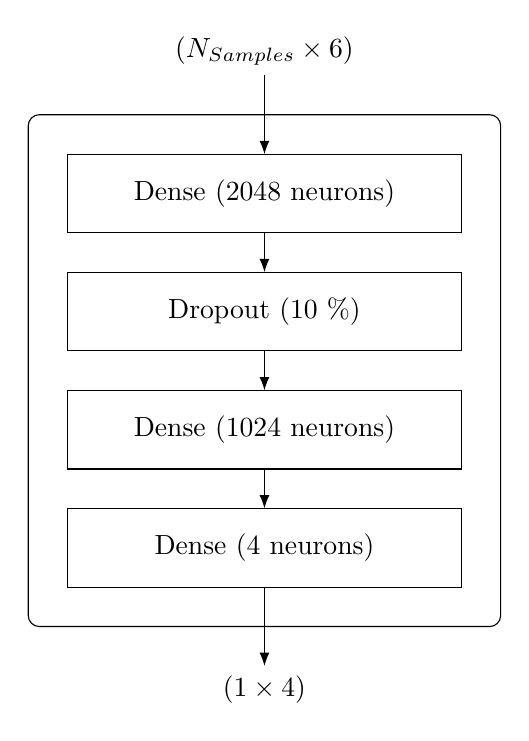
\begin{tikzpicture}
        \draw[rounded corners] (0,0) rectangle (6,-6.5); \draw[Latex-] (3,-0.5)
        -- ++(0,1) node[above] {$\left(N_{Samples} \times 6\right)$};


        \draw (0.5,-0.5) coordinate (tmp) rectangle ++(5,-1); \node () at
        ($(tmp) + (2.5, -0.5)$) {Dense ($2048$ neurons)};

        \draw[-Latex] ($(tmp) + (2.5,-1)$) -- ++(0,-0.5);

        \draw (0.5,-2) coordinate (tmp) rectangle ++(5,-1); \node () at ($(tmp)
        + (2.5, -0.5)$) {Dropout ($10\ \si{\percent}$)};

        \draw[-Latex] ($(tmp) + (2.5,-1)$) -- ++(0,-0.5);

        \draw (0.5,-3.5) coordinate (tmp) rectangle ++(5,-1); \node () at
        ($(tmp) + (2.5, -0.5)$) {Dense ($1024$ neurons)};

        \draw[-Latex] ($(tmp) + (2.5,-1)$) -- ++(0,-0.5);

        \draw (0.5,-5) coordinate (tmp) rectangle ++(5,-1); \node () at ($(tmp)
        + (2.5, -0.5)$) {Dense ($4$ neurons)};

        \draw[-Latex] ($(tmp) + (2.5,-1)$) -- ++(0,-1) node[below]
        {$\left(1\times 4\right)$};
        
        
    \end{tikzpicture}
    \caption{The architecture of the head-model. All layers except the last one
    use \textit{ReLU}-activation. The output-layer uses
    \textit{softmax}-activation.}
    \label{fig:head-model}
\end{figure}

\begin{figure}[htbp]
    \centering
    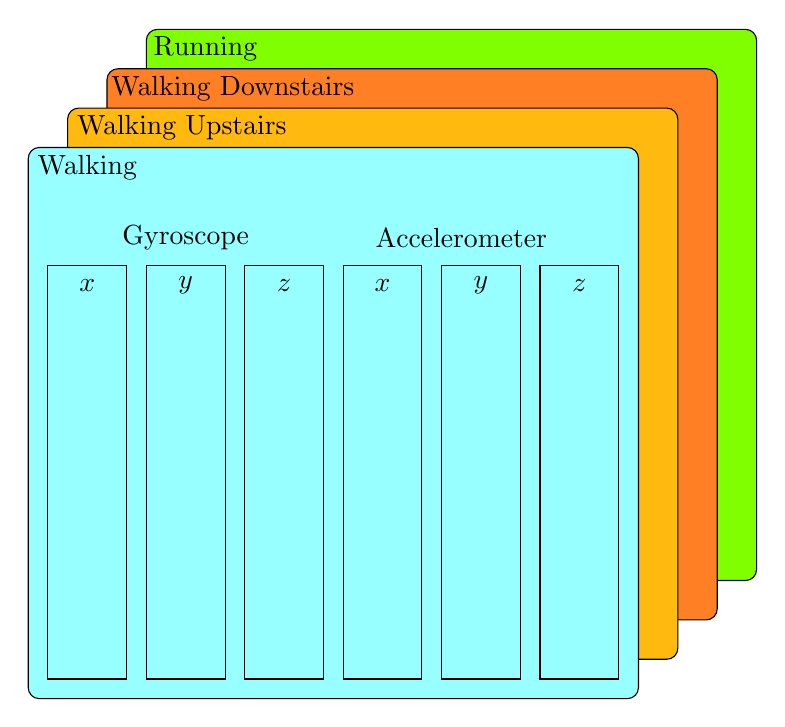
\begin{tikzpicture}

        \draw[fill=Chartreuse1, rounded corners] (2,0) rectangle(9.75,7); \node
        () at (2.75, 6.75) {Running};

        \draw[fill=Chocolate1, rounded corners] (1.5, -0.5) rectangle (9.25,
        6.5); \node () at (3.1, 6.25) {Walking Downstairs};

        \draw[fill=DarkGoldenrod1, rounded corners] (1, -1) rectangle (8.75, 6);
        \node () at (2.45, 5.75) {Walking Upstairs};

        \draw[fill=DarkSlateGray1, rounded corners] (0.5, -1.5) rectangle (8.25,
        5.5); \node () at (1.25, 5.25) {Walking};

        \draw (0.75, 4) rectangle ++(1,-5.25); \draw (2, 4) rectangle
        ++(1,-5.25); \draw (3.25, 4) rectangle ++(1,-5.25); \draw (4.5, 4)
        rectangle ++(1,-5.25); \draw (5.75, 4) rectangle ++(1,-5.25); \draw (7,
        4) rectangle ++(1,-5.25);

        \node () at (2.5, 4.35) {Gyroscope}; \node () at (6, 4.35)
        {Accelerometer};

        \node () at (1.25, 3.75) {$x$}; \node () at (2.5, 3.75) {$y$}; \node ()
        at (3.75, 3.75) {$z$}; \node () at (5, 3.75) {$x$}; \node () at (6.25,
        3.75) {$y$}; \node () at (7.5, 3.75) {$z$};
    \end{tikzpicture}
    \caption{Architecture of 2D convolution-layer. The sensor-data is
    interpreted by an $N_{Samples} \times 6$ image. As a $4$-seconds timeframe
    at a sampling-rate of $50 \si{\hertz}$ is chosen in the pre-processing, one
    derives $N_{Samples} = 200$. The 2D-convolution is set up to have $4$
    channels, resulting in an own convolution channel for each activity.}
    \label{fig:conv_2d_arch}
\end{figure}

\begin{figure}[htbp]
    \centering
    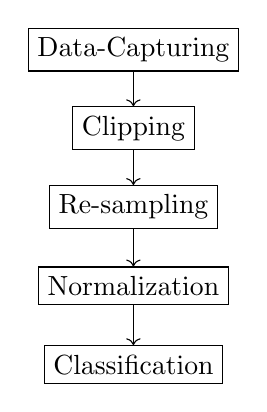
\begin{tikzpicture}
        \node[draw] (capturing) at (0,0) {Data-Capturing}; 
        \node[draw] (clipping) at (0,-1) {Clipping}; 
        \node[draw] (resampling) at (0,-2) {Re-sampling}; 
        \node[draw] (normalize) at (0,-3) {Normalization};
        \node[draw] (classify) at (0,-4) {Classification};

        \graph[nodes={draw}] {(capturing) -> (clipping) -> (resampling) ->
            (normalize) -> (classify);};
    \end{tikzpicture}
    \caption{Outline of transfer-learning signal-processing pipeline.}
    \label{fig:TFL_signal_processing}
\end{figure}

\section{Validating parent- and child-model}
Although the child-model is actually trained on-device, an offline-training and
validation procedure was set-up during the development process to validate its 
classification-performance. The
confusion-matrices for both, parent- and child-models for the already introduced
data-sets (figures \ref{fig:hist_parent_training} to \ref{fig:hist_child_validation}) 
are shown in figures \ref{fig:parent_confusion_matrix} and
\ref{fig:child_confusion_matrix}.

\begin{figure}
    \centering
    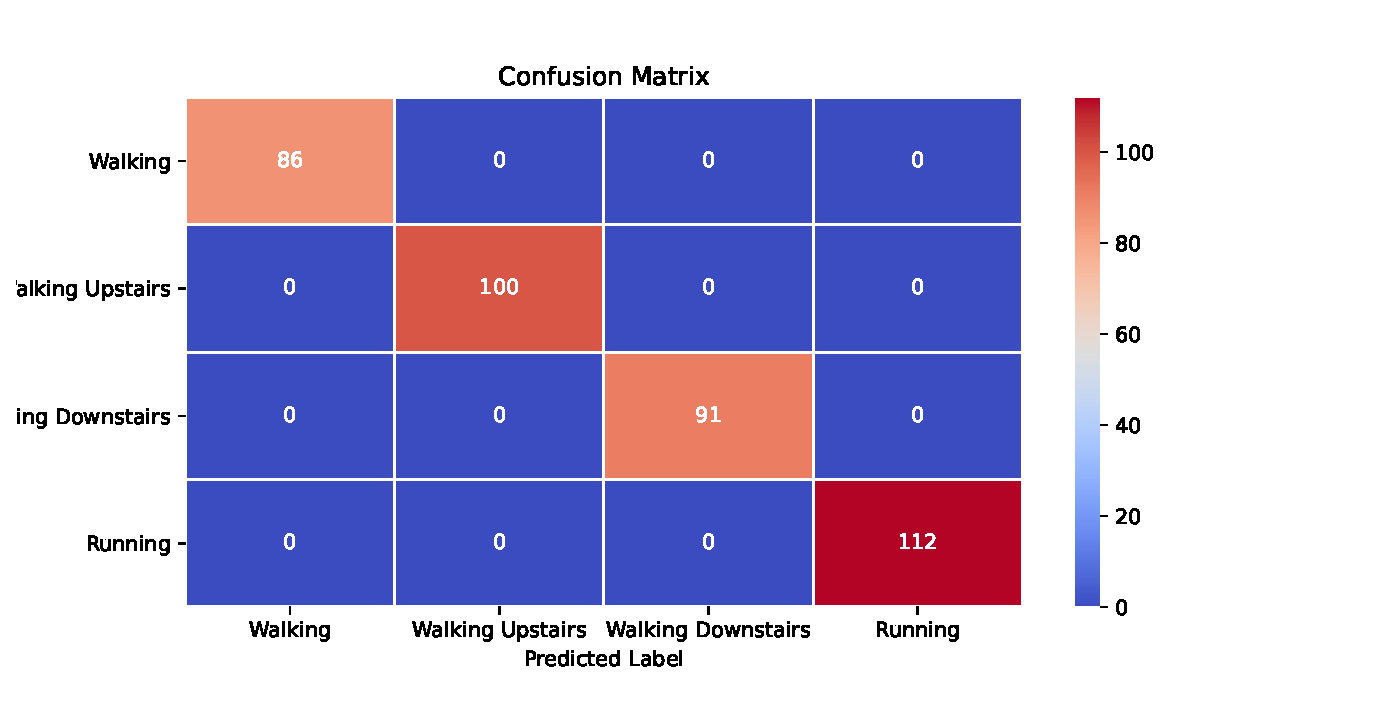
\includegraphics[width=0.5\textwidth]{figures/parent_confusion_matrix.eps}
    \caption{Confusion-matrix of the parent-model.}
    \label{fig:parent_confusion_matrix}
\end{figure}


\begin{figure}
    \centering
    \includegraphics[width=0.5\textwidth]{figures/child_confusion_matrix.eps}
    \caption{Confusion-matrix of the child-model.}
    \label{fig:child_confusion_matrix}
\end{figure}

\section{The App UI}
This section gives an quick introduction on the UI of the app.\newline
After opening the app, the user observes the UI-window shown in figure\ref{fig:UI_main}.
He can then choose between the 3 actions:
\begin{itemize}
    \item \textbf{CAPTURE DATA (Figure \ref{fig:UI_data_capturing})}: \newline
    This button opens a new window for capturing the sensor-data and storing it to a 
    \textit{.csv}-file on the device. Thereby, the selected activity only
    affects the names of the resulting files, so one can keep the default selection
    when not caring about the actual name of the output file.
    To prevent overwriting previous captures, a suffix is attached to the single filenames
    containing the UTC-timestamp from the start of the capture in milliseconds. 

    \item \textbf{ACTIVITY RECOGNITION KNN (Figure \ref{fig:UI_kNN})}:\newline
    This button opens a window
    for classifying an activity with the pre-trained \textit{kNN}-classifier. 
    The classification is executed continuously as soon as this window is opened.

    \item \textbf{TRANSFER LEARNING (Figure \ref{fig:UI_TFL})}:\newline
    This window contains all possible actions for the transfer-learning
    part of the app. The upper part shows the probabilities of the single classes
    as well as the class with the currently highest probability.
    Classification is not started when the window is opened, but has to be
    manually enabled through the \textit{Inference}-switch. \newline

    The lower section contains all actions and information about the
    transfer-learning samples themselves. Similar as in the data-capturing
    window, the user can select the proper activity and start the recording
    via the \textit{Record}-switch.\newline
    The table below this switch shows a summary of the captured samples:
    How much samples were captured and when they were updated. Through the
    switch with labels \textit{Overwrite} and \textit{Add}, the user
    can select whether to overwrite the samples for the selected activity
    after the next capture, or to add new samples.\newline
    The \textit{DEBUG} button automatically loads the validation-set shown earlier
    in this report. This functionality can be used for debugging and validation purposes.\newline
    The actual learning procedure is then started via the \textit{Learn}-switch. Thereby, the current
    loss is additionally printed right next to the switch.\newline
    When disabling the learning, the current optimization-epoch is finished, so it is recommended 
    to wait a few seconds until the loss-value is updated to its final value.
    

\end{itemize}
\begin{figure}[htbp]
    \centering
    \includegraphics[width=0.2\textwidth]{figures/UI_main.jpg}
    \caption{The main-window, seen by the user when opting the app.}
    \label{fig:UI_main}
\end{figure}

\begin{figure}[htbp]
    \centering
    \includegraphics[width=0.2\textwidth]{figures/UI_data_capturing.jpg}
    \caption{The UI-window for capturing data.}
    \label{fig:UI_data_capturing}
\end{figure}

\begin{figure}[htbp]
    \centering
    \includegraphics[width=0.2\textwidth]{figures/UI_kNN.jpg}
    \caption{The UI-window for the \textit{kNN}-classifier.}
    \label{fig:UI_kNN}
\end{figure}

\begin{figure}[htbp]
    \centering
    \includegraphics[width=0.2\textwidth]{figures/UI_TFL.jpg}
    \caption{The UI-window for the transfer-learning part of the assignment.}
    \label{fig:UI_TFL}
\end{figure}

\section{Issues, Possible Improvements and Conclusion}
\label{sec:conclusion}
The main reason why a different set of activities was chosen for part 1 and part
2 is, that it was originally planned to use a provided data-set for
transfer-learning, containing the 6 activities \textit{Walking}, \textit{Walking
Upstairs}, \textit{Walking Downstairs}, \textit{Standing}, \textit{Sitting},
\textit{Laying} as well as the 6 activity-transitions \textit{Stand-to-Sit},
\textit{Sit-to-Stand}, \textit{Sit-to-Lay}, \textit{Lay-to-Sit},
\textit{Stand-to-Lay} and \textit{Lay-to-Stand}. Later, the
\textit{kNN}-classifier should also be trained and applied to these
activities/activity-transitions. Unfortunately, designing and
implementing a model for this $12$ classes were harder then expected, especially
as the originally used phone had a broken accelerometer. As the activities in
part 1 are mainly characterized by their axis of rotation, a accurate
classification was possible, independent of the accelerometer. The broken
sensor then became a real problem when testing a first version of the
parent-model, which achieved a quite acceptable accuracy on the computer, but
had a terrible performance when utilizing it on the phone. \newline
To determine whether this issue is data-set of phone-related, an own data-set for
the 4 activities then finally implemented in the app was collected. After a
quite large time invested in debugging, the accelerometer could finally be recognized
as the actual cause of the problem. \newline
After a new phone was obtained, the reduced data-set was re-collected and
parent- and child-models were re-designed, implemented and tested, no time was
available anymore to switch from the two self-collected data-sets for the two
different sets of activities, to the provided data-set with its 6 activities and
6 activity-transition. Instead, stability and performance of the app and the
derived results were optimized.\newline

One issue observed while designing and testing the current 4-activity data-set
was that the performance of the transfer-learning model significantly depends
on the phone itself as well as its position: When wearing 'loose' trousers, 
the phone starts to jump-around within the pocket in an non-deterministic way 
for several activities. This, of course, makes it hard for the model to 
determine the correct activity. 
This problem especially occurs when putting the phone in one of the back pockets, 
as these are typically looser than front-pockets. 
Further, size and weight of phone significantly increased during the past years.
This facts further promote the jumping.\newline

To conclude, the classifiers for both parts of this assignment work as expected.
One could definitely improve the number of activities to recognize as well as
utilizing \textit{kNN-} and \textit{transfer-learning} classifiers to the same
activity-set. Further, one could try to train the \textit{transfer-learning}
classifier on a data-set captured really by different phones, as this would
further generalize the approach. Further, the number of parameters for the
\textit{transfer-learning} model might be reduced to improve the
training-performance on older phones. 




\section{Appendix}

\printbibliography

\end{document}
